\chapter{Apéndice D. Códigos desarrollados.}

\subsection{Códigos del módulo de Seguimiento Solar}

\subsubsection{Programa en Mathematica para obtener la velocidad angular máxima y la potencia teóricas para los motores de movimiento elevación y azimutal.}

\UseRawInputEncoding
\lstinputlisting[language=Mathematica]{PolinomioTrayectoria.txt}

\subsubsection{Programa en Mathematica para obtener las matrices de la cinemática directa y dinámica del robot seguidor.}

\UseRawInputEncoding
\lstinputlisting[language=Mathematica]{modeloCinematicoDinamico.txt}

\subsubsection{Programa en MATLAB para calcular los parámetros físicos del motor.}

\UseRawInputEncoding
\lstinputlisting[language=Matlab]{parametrosMotor.m}

\subsubsection{Función en MATLAB que contiene la programación de las ecuaciones del modelo dinámico del robot seguidor.}

\UseRawInputEncoding
\lstinputlisting[language=Matlab]{fcnDinamicaRobot.m}

\subsubsection{Programa en MATLAB que toma los datos generados por los diagramas de bloques de los controladores para calcular los valores máximos de las variables más importantes del sistema.}

\UseRawInputEncoding
\lstinputlisting[language=Matlab]{parametrosMaximos.m}

\subsection{Códigos del módulo Estructural}

\subsubsection{Código en MATLAB con las instrucciones principales de la interfaz gráfica para el cálculo de perfiles estructurales.}

\UseRawInputEncoding
\lstinputlisting[language=Matlab, linerange={47-86,137-255,365-551}]{analisisResistencia.m}

\subsubsection{Programa en MATLAB para el cálculo de la sección transversal del tubo de soporte principal.}

\UseRawInputEncoding
\lstinputlisting[language=Matlab]{columnaAnalisis.m}

\subsubsection{Programa en MATLAB para validar la resistencia teórica del brazo de soporte auxiliar.}

\UseRawInputEncoding
\lstinputlisting[language=Matlab]{analisisBrazoSoporte.m}

\subsection{Códigos del módulo de Mando Central}

\subsubsection{Programa en MATLAB para generar las gráficas de la trayectoria solar y la simulación del robot utilizando las ecuaciones de cinemática directa.}

\UseRawInputEncoding
\lstinputlisting[language=Matlab]{modeloCinematico.m}

\subsubsection{Código del servidor web en HTML}

\begin{figure}[H]
	\centering
	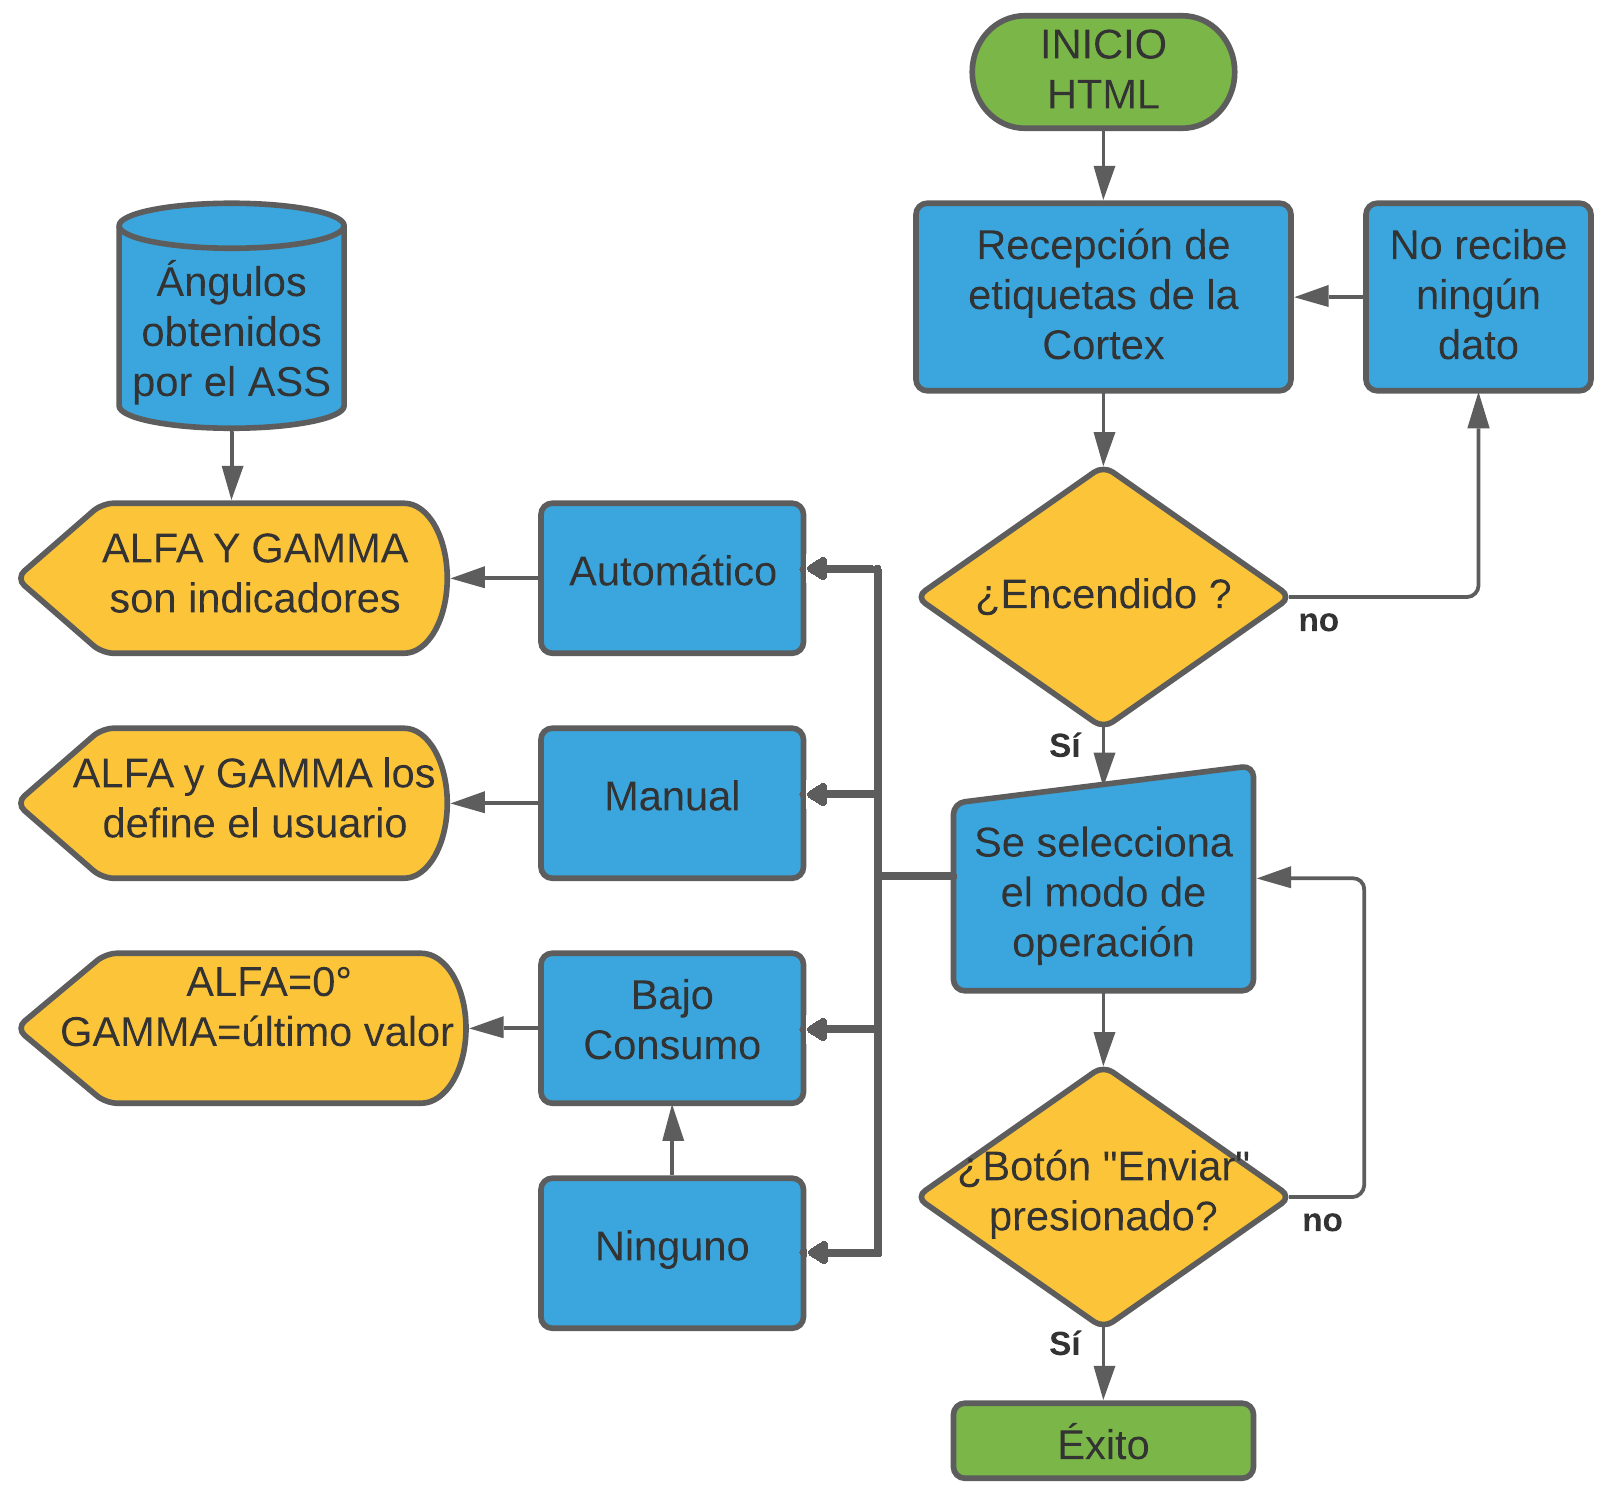
\includegraphics[width=\columnwidth]{imagenes/Diagrama HTML.png}
	\caption{Diagramas de flujo del código HTML}
	\label{fig:dia_flujHTML}
\end{figure}

\subsubsection{Código de la NUCLEO en C}

\begin{figure}[H]
	\centering
	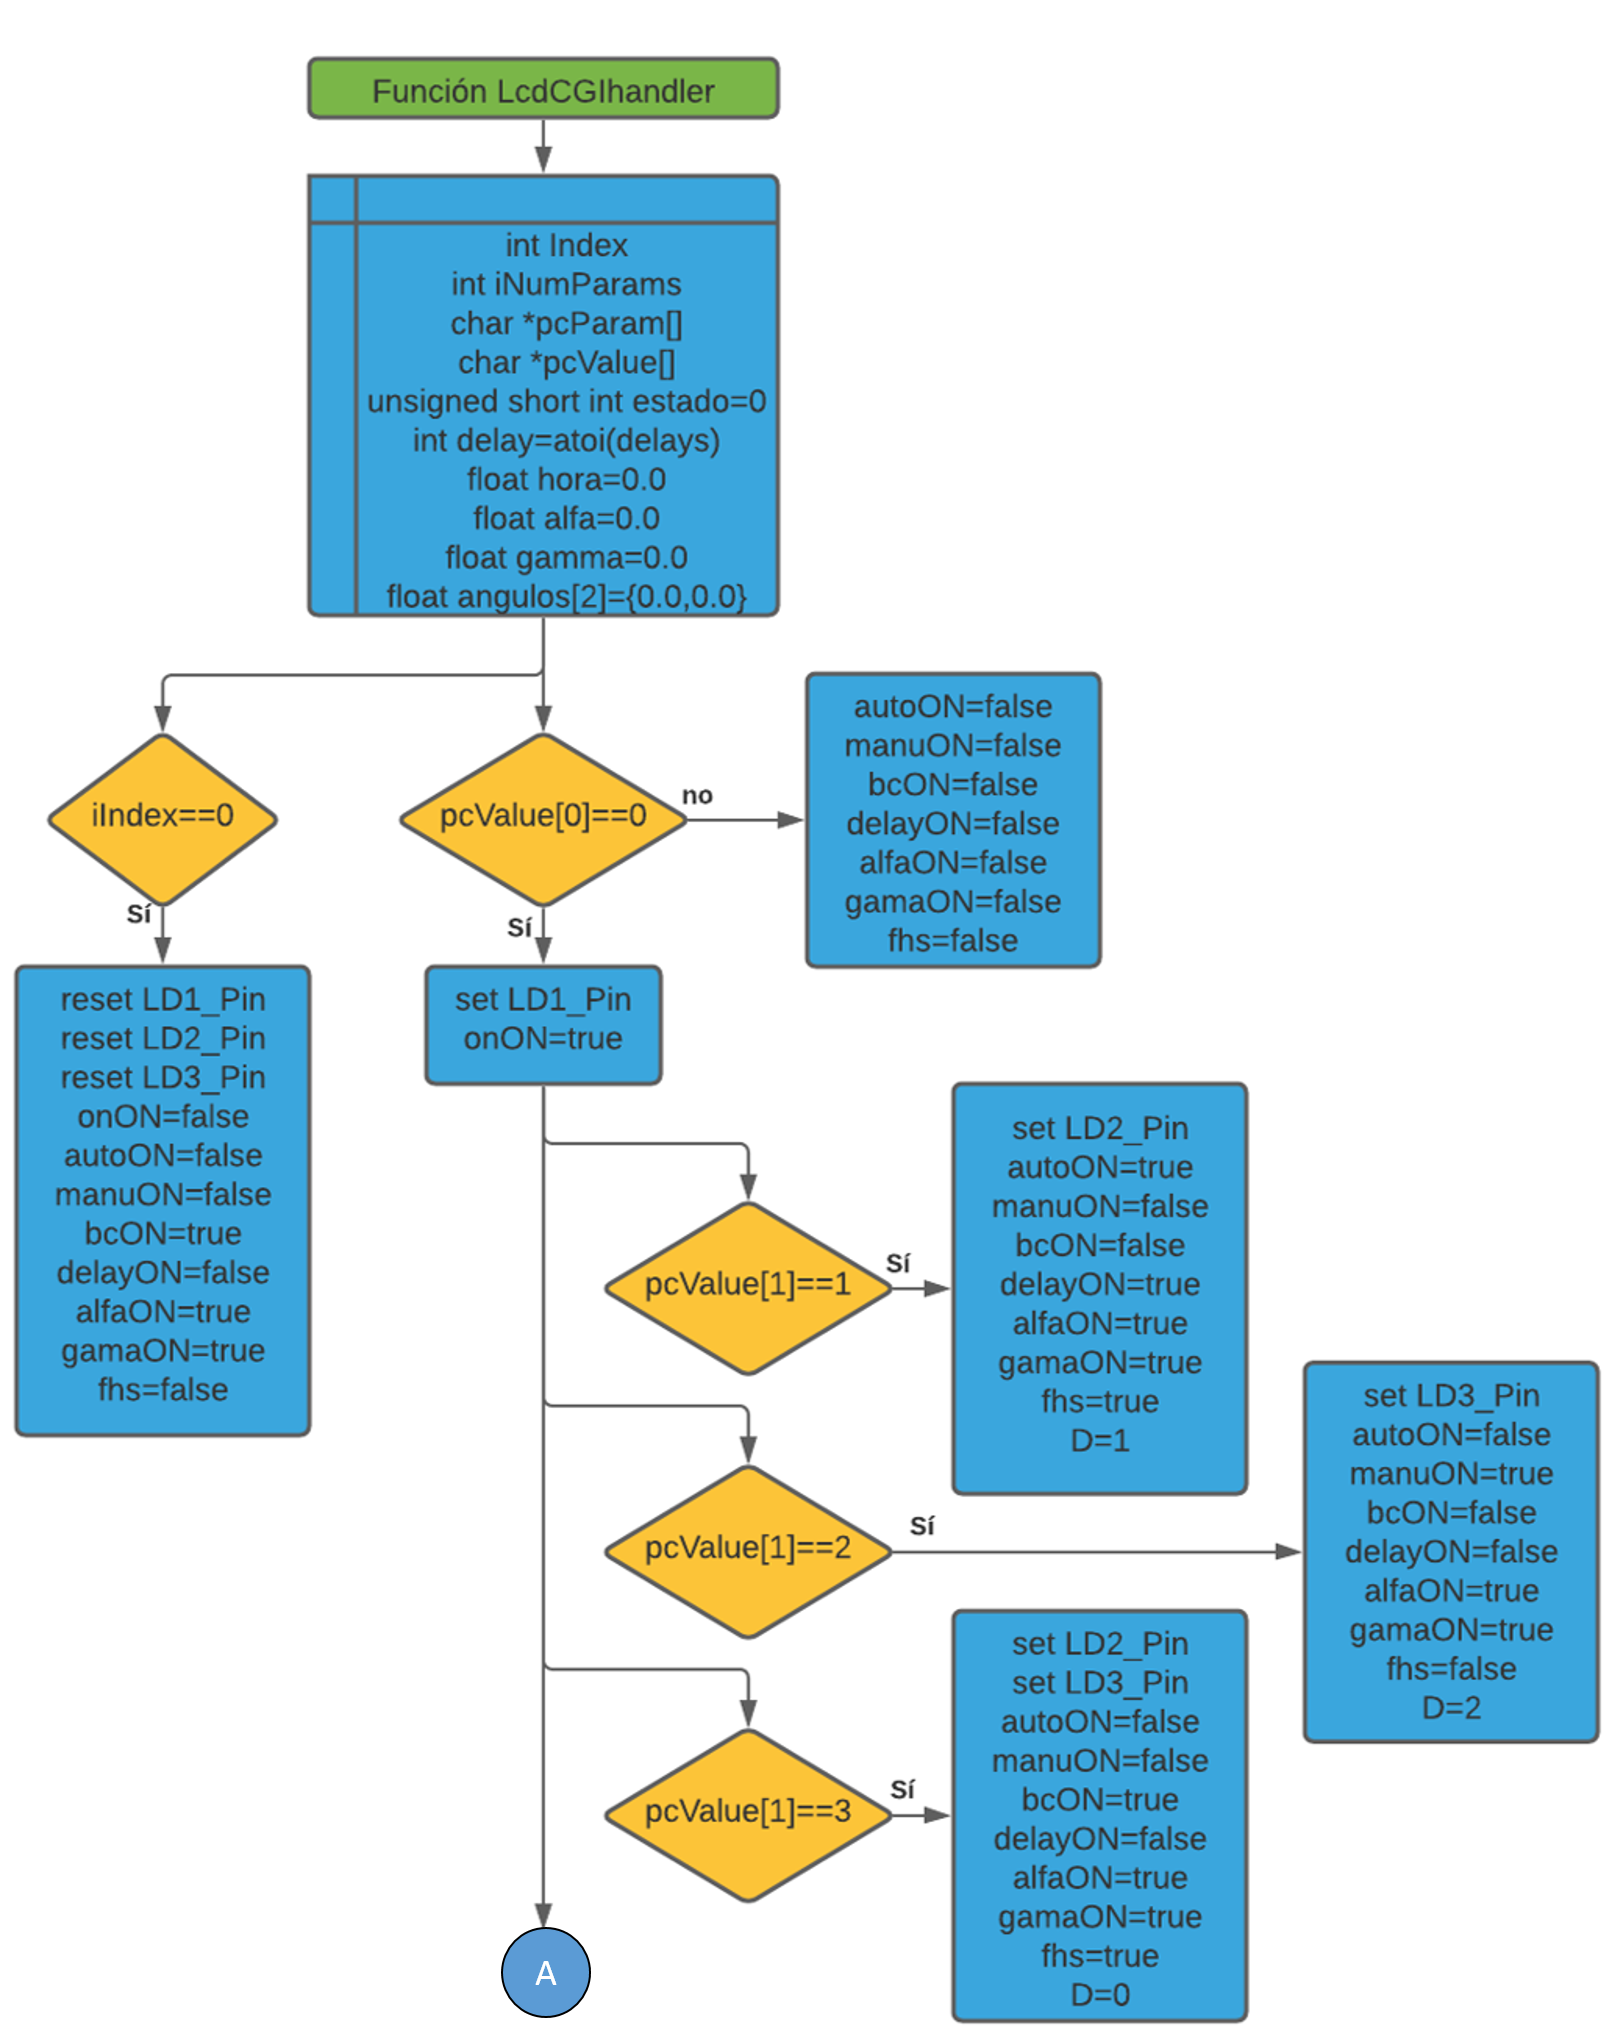
\includegraphics[width=\columnwidth]{imagenes/Diagrama CGI 1.png}
	\caption{Diagrama de flujo del código CGI (1)}
	\label{fig:dia_flujCGI1}
\end{figure}

\begin{figure}[H]
	\centering
	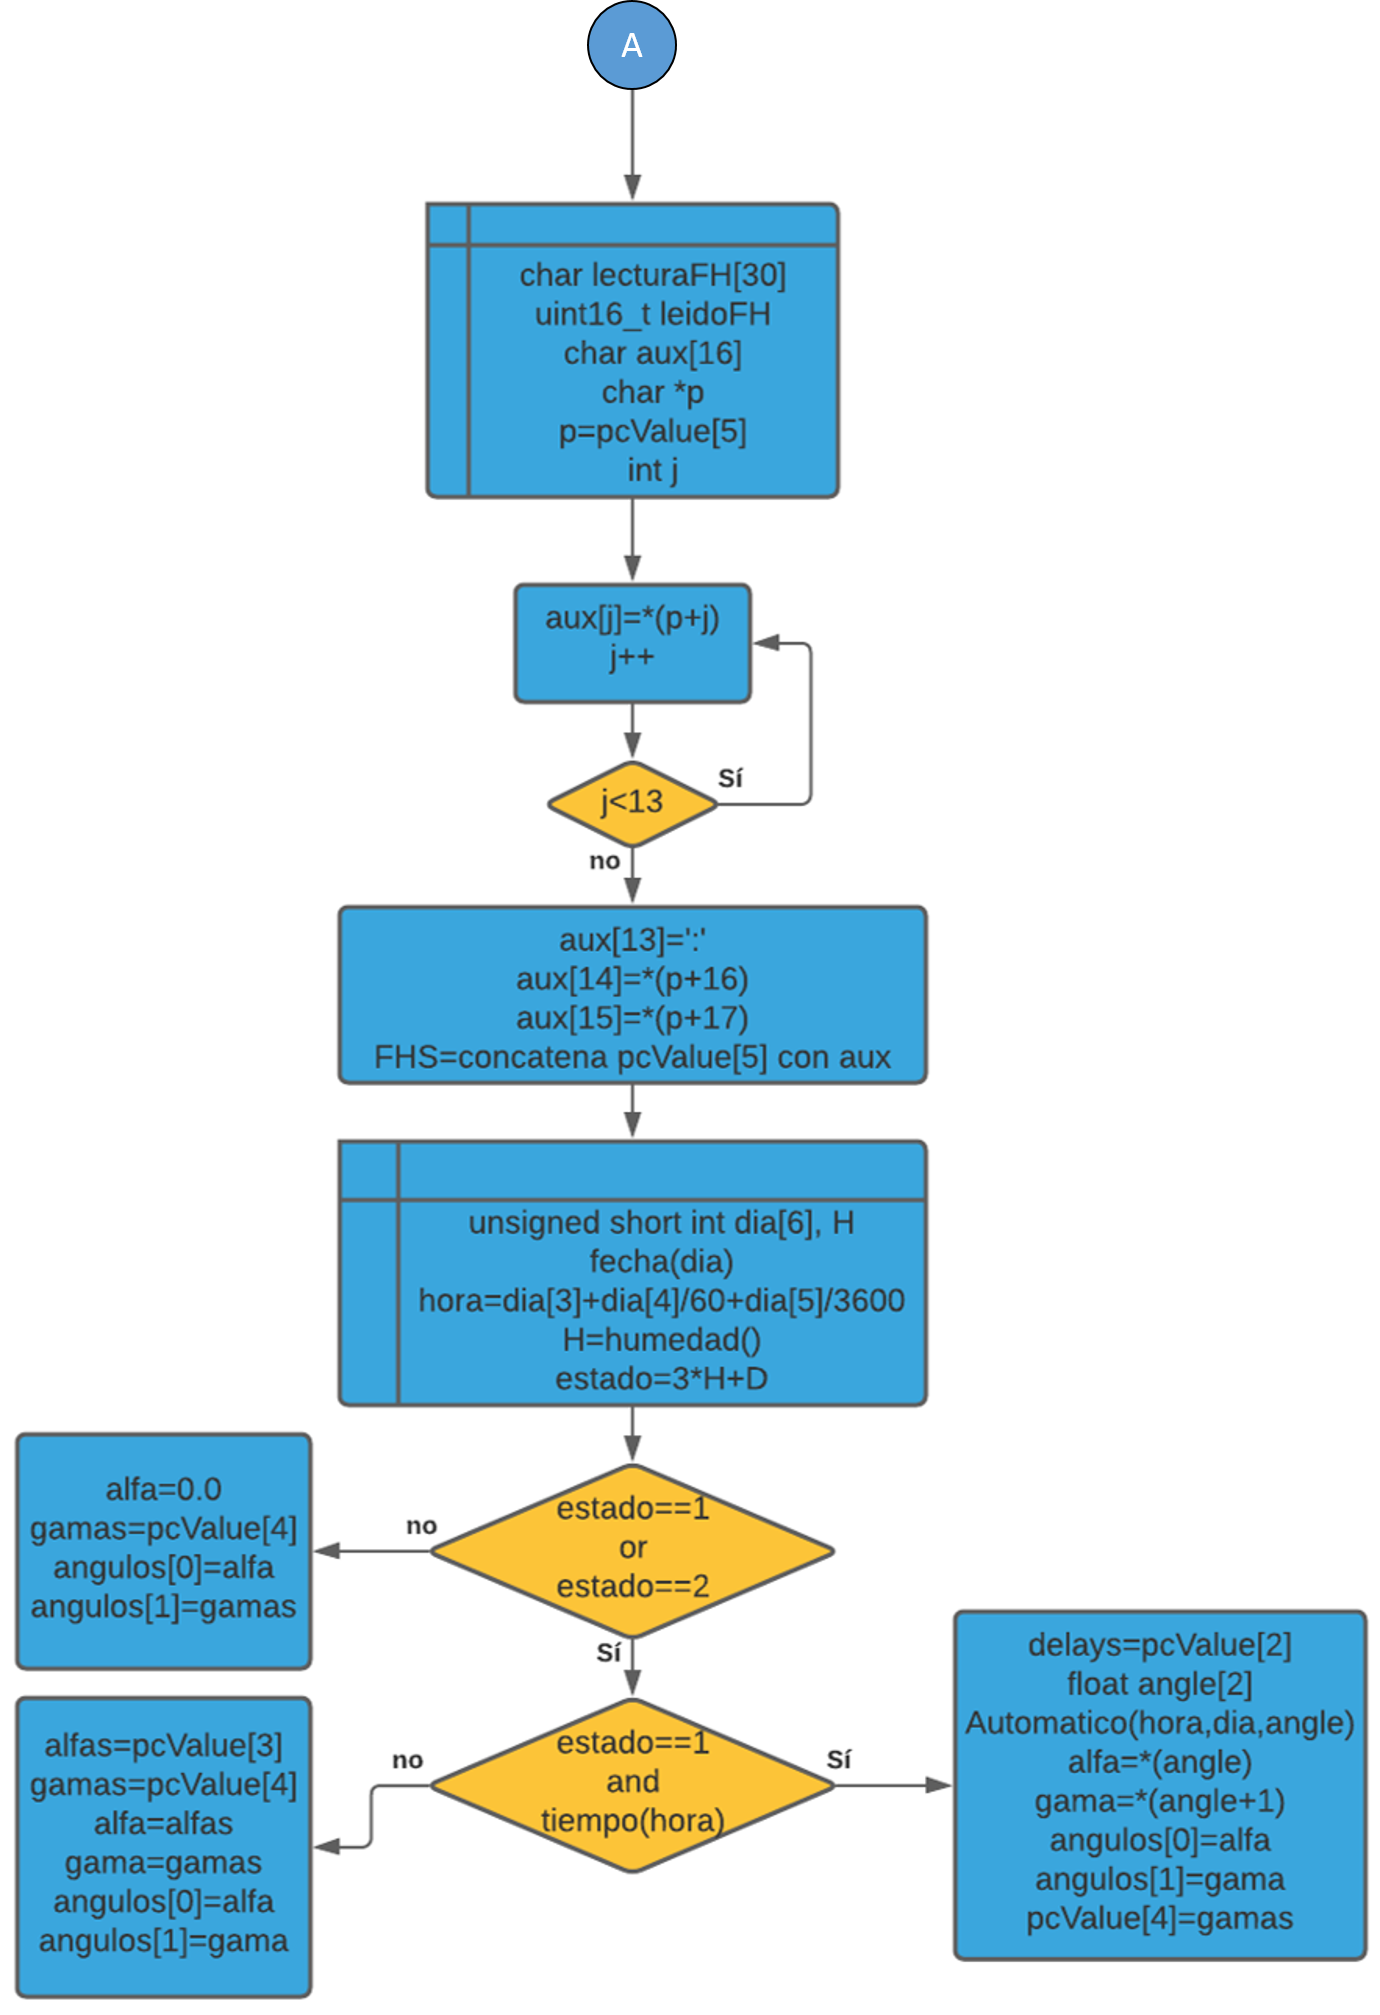
\includegraphics[width=\columnwidth]{imagenes/Diagrama CGI 2.png}
	\caption{Diagrama de flujo del código CGI (2)}
	\label{fig:dia_flujCGI2}
\end{figure}

\begin{figure}[H]
	\centering
	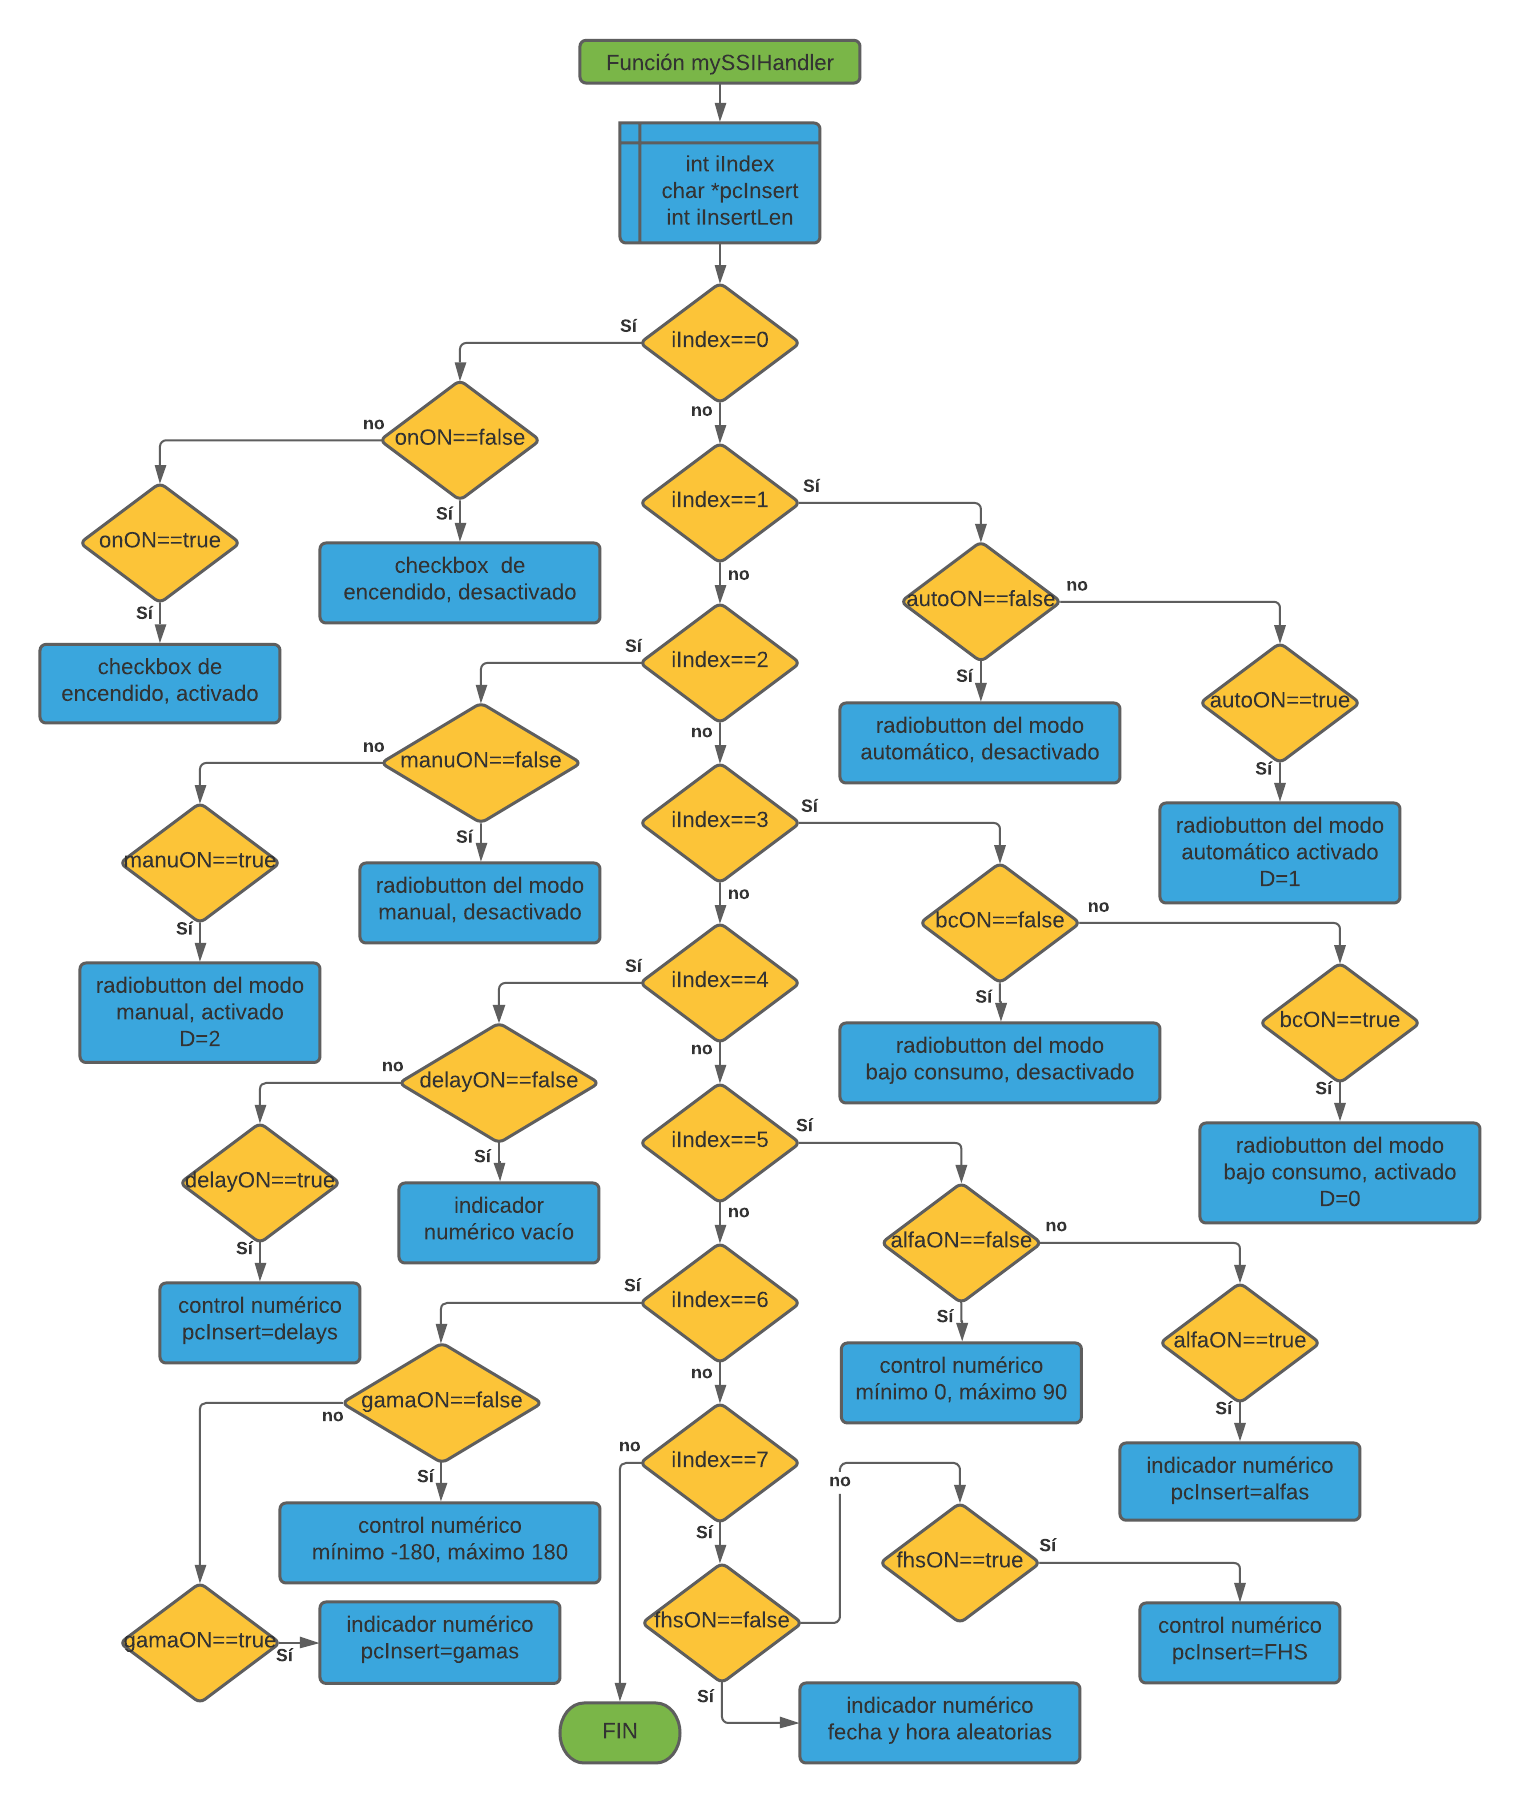
\includegraphics[width=\columnwidth]{imagenes/Diagrama SSI.png}
	\caption{Diagrama de flujo del código SSI}
	\label{fig:dia_flujSSI}
\end{figure}






\bigskip

%%%%%%fin del archivo
\endinput 